\section{Cipher Specifications}

\begin{frame}{Specifications}
    \begin{itemize}
        \item Three members of Loong cipher: \textbf{Loong-64}, \textbf{Loong-80} and \textbf{loong-128}
        \pause
        \item Block size of Loong is 64-bit
        \pause
        \item Number of rounds are 16, 20 and 32 for 64-bit, 80-bit and 128-bit key respectively.
    \end{itemize}
\end{frame}

\begin{frame}{Encryption}
    \begin{figure}[htp]
    \centering
    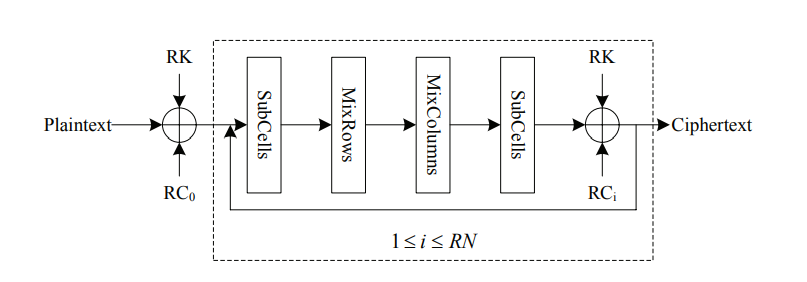
\includegraphics[width=10cm]{encrypt.png}
    \caption{Encryption Function}
    \label{fig:encryption-function}
    \end{figure}
\end{frame}

\begin{frame}{Subcells}
    \begin{table}[H]
    	\begin{center}
    	\scalebox{0.8}{
    	\begin{tabular}{||c||c|c|c|c|c|c|c|c|c|c|c|c|c|c|c|c|}
    		\hline
    		x & 0 & 1 & 2 & 3 & 4 & 5 & 6 & 7 & 8 & 9 & A & B & C & D & E & F\\ 
    		\hline
    		S(x) & C & A & D & 3 & E & B & F & 7 & 9 & 8 & 1 & 5 & 0 & 2 & 4 &6\\
    		\hline
    	\end{tabular}}
    	\end{center}
    	\caption{S-Box}
    	\label{table:sbox}
    \end{table}
    \begin{itemize}
        \item Special property of \textbf{involutive} in the SBox
        \pause
        \item It means the S-Box is its own inverse.
        \pause
        \item x = S(S(x))
    \end{itemize}
\end{frame}
    
\begin{frame}{MixRows}
    \begin{itemize}
        \item  In MixRow Operation, the state is post-multiplied by a diffusion matrix $M$. 
        \pause
        \item The matrix multiplication is performed in finite field $GF(2^4)$ where the irreducible polynomial is $x^4 + x+ 1$.
    \end{itemize}
    \begin{align*}
    state \leftarrow 
    \begin{pmatrix}
    state_0 & state_1 & state_2 & state_3 \\
    state_4 & state_5 & state_6 & state_7 \\
    state_8 & state_{9} & state_{10} & state_{11} \\
    state_{12} & state_{13} & state_{14} & state_{15}
    \end{pmatrix}
    \times
    \begin{pmatrix}
    1 & 4 & 9 & 13\\
    4 & 1 & 13 & 9\\
    9 & 13 & 1 & 4\\
    13 & 9 & 4 & 1
    \end{pmatrix}
    \end{align*}
\end{frame}

\begin{frame}{MixColumns}
    \begin{itemize}
        \item In MixColumn Operation, the state is pre-multiplied by a diffusion matrix $M^'$. 
        \pause
        \item The matrix multiplication is performed in finite field $GF(2^4)$ where the irreducible polynomial is $x^4 + x+ 1$.
    \end{itemize}
    \begin{align*}
    state \leftarrow 
    \begin{pmatrix}
    13 & 9 & 4 & 1\\
    9 & 13 & 1 & 4\\
    4 & 1 & 13 & 9\\
    1 & 4 & 9 & 13
    \end{pmatrix}
    \times
    \begin{pmatrix}
    state_0 & state_1 & state_2 & state_3 \\
    state_4 & state_5 & state_6 & state_7 \\
    state_8 & state_{9} & state_{10} & state_{11} \\
    state_{12} & state_{13} & state_{14} & state_{15}
    \end{pmatrix}
    \end{align*}
\end{frame}

\begin{frame}{Round Constants}
    \begin{itemize}
        \item 6-bit affine linear-feedback shift register(LFSR)
        \begin{align*}
        (rc_5, rc_4, rc_3, rc_2, rc_1, rc_0) \leftarrow (rc_4, rc_3, rc_2, rc_1, rc_0, rc_5 \oplus rc_4 \oplus 1)
        \end{align*}
        \pause
        \item Round Constants are intialized to 0.
        \pause
        \item The adding(XOR) of the round constants in the AddRoundKey is arranged as follows:\\
        \begin{center}
            $\begin{bmatrix}
        0 & 0 & 0 &(rc_5 || rc_4 || rc_3)\\
        0 & 0 & 1 &(rc_2 || rc_1 || rc_0)\\
        0 & 0 & 2 &(rc_5 || rc_4 || rc_3)\\
        0 & 0 & 4 &(rc_2 || rc_1 || rc_0)
        \end{bmatrix}$
        \end{center}
    \end{itemize}
\end{frame}

\begin{frame}{AddRoundKey}
    The 64-bit key of Loong-64 is arranged into a round key matrix as:\\
    \begin{center}
    $ RK \leftarrow 
    \begin{bmatrix}
    k_0 & k_1 & k_2 & k_3 \\
    k_4 & k_5 & k_6 & k_7 \\
    k_8 & k_9 & k_{10} & k_{11} \\
    k_{12} & k_{13} & k_{14} & k_{15}
    \end{bmatrix}$
    \end{center}
\end{frame}
\begin{frame}{AddRoundKey}
    The 80-bit key of Loong-80 is arranged into two round key matrix:\\
    \begin{center}
    $ RK_0 \leftarrow 
    \begin{bmatrix}
    k_0 & k_1 & k_2 & k_3 \\
    k_4 & k_5 & k_6 & k_7 \\
    k_8 & k_9 & k_{10} & k_{11} \\
    k_{12} & k_{13} & k_{14} & k_{15}
    \end{bmatrix} \hspace{1cm}
    RK_1 \leftarrow 
    \begin{bmatrix}
    k_{16} & k_{17} & k_{18} & k_{19}\\
    k_0 & k_1 & k_2 & k_3 \\
    k_4 & k_5 & k_6 & k_7 \\
    k_8 & k_9 & k_{10} & k_{11}
    \end{bmatrix}$
    \end{center}
\end{frame}
\begin{frame}{AddRoundKey}
    The 128-bit key of Loong-128 is arranged into two round key matrix as:\\
    \begin{center}
    $ RK_0 \leftarrow 
    \begin{bmatrix}
    k_0 & k_1 & k_2 & k_3 \\
    k_4 & k_5 & k_6 & k_7 \\
    k_8 & k_9 & k_{10} & k_{11} \\
    k_{12} & k_{13} & k_{14} & k_{15}
    \end{bmatrix} \hspace{1cm}
    RK_1 \leftarrow 
    \begin{bmatrix}
    k_{16} & k_{17} & k_{18} & k_{19}\\
    k_{20} & k_{21} & k_{22} & k_{23} \\
    k_{24} & k_{25} & k_{26} & k_{27} \\
    k_{28} & k_{29} & k_{30} & k_{31}
    \end{bmatrix}$
    \end{center}
\end{frame}
\begin{frame}{AddRoundKey}
    For 64-bit key, the AddRoundKey operation is as:
    \begin{equation}
        state \leftarrow state \oplus RK \oplus RC_{i} \hspace{10pt}
        (0 \leq i \leq RN)     
    \end{equation}
    For 80-bit and 128-bit key, the AddRoundKey Operation is as:\\
    \begin{equation}
        state \leftarrow state \oplus RK_{i\;mod\;2} \oplus RC_{i}
        \hspace{10pt}
        (0 \leq i \leq RN) 
    \end{equation}
\end{frame}

\begin{frame}{Decryption}
    \begin{figure}[htp]
    \centering
    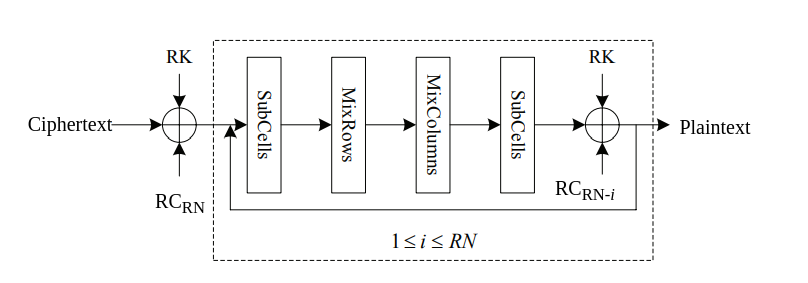
\includegraphics[width=10cm]{decrypt.png}
    \caption{Decryption Function}
    \label{fig:encryption-function}
\end{figure}
\end{frame}

\begin{frame}{Comparison Between Encryption \& Decryption}
    \begin{figure}[ht]
        \begin{minipage}[b]{0.45\linewidth}
            \centering
            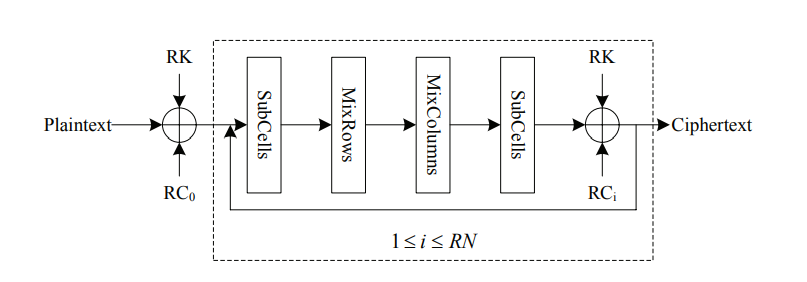
\includegraphics[width=6cm]{encrypt.png}
            \caption{Encryption Process}
            \label{fig:a}
        \end{minipage}
        \hspace{0.5cm}
        \begin{minipage}[b]{0.45\linewidth}
            \centering
            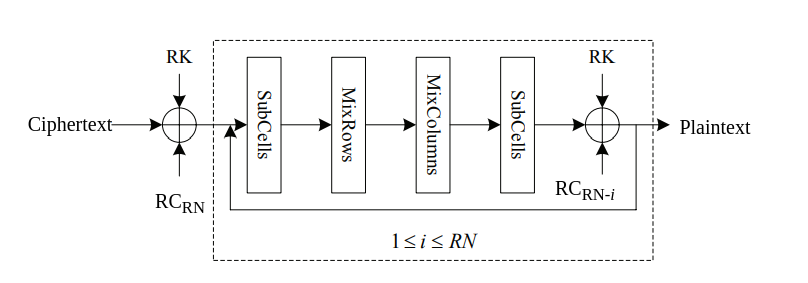
\includegraphics[width=6cm]{decrypt.png}
            \caption{Decryption Process}
            \label{fig:b}
        \end{minipage}
        % 
        \caption{Similar Encryption and decryption Process}
    \end{figure}
    The process of Decryption is same as encryption in Loong. The only difference is round constants are used in reverse order.
\end{frame}

\begin{frame}{Why Loong?}
    \begin{itemize}
        \item Encryption and decryption process is same.
        \pause
        \item Easy to implement on hardware.
        \pause
        \item Provides Two times confusion in one round of cipher.
        \pause
        \item Highly security against cryptanalysis, especially the
differential attack and linear attack.
    \end{itemize}
\end{frame}
